\chapter{Evaluation}

\section{Generated Datasets}

After filtering the template images manually using the Filtering Tool and
the methodology described in Chapter 4, a total of 361 template images were
selected.

Using the Canny2Concrete pipeline with these filtered template images,
\emph{GARD} was generated, containing a total of 45486 images, separated
into three datasets:

\begin{enumerate}
\item \texttt{BaseImages}: containing 6498 images (18 variations for each of the 361 canny edge images).
\item \texttt{VariantImages}: containing 19494 images (3 variations for each base image) \emph{before} weather occlusion.
\item \texttt{VariantImagesWithOcclusion}: also 19494 images, same as \texttt{VariantImages} but with weather effects applied.
\end{enumerate}

\section{Sample Images}

To demonstrate a sample of generated images, three random template images were
chosen. Two are close-up shots and the third is a far away picture. They
are shown as three grids of images of for rows.

The first row contains the template image, the canny edge extracted from it,
and the runway label mask. The second row contains three images from the Base
Images dataset generated from the template image. The third row contains three
images from the Variant Images dataset, generated from the Base Images. The
fourth row contains three images from the Variant Images with Occlusion dataset,
associated with the shown Variant Images.

\begin{figure}[htbp]
\centering
\includegraphics[width=1.2\textwidth]{figures/GeneratedImage1.png}
  \caption{Images generated from the template image \emph{"9xG0a8TUdXg\_028"} }
\label{fig:noise_to_image}
\end{figure}

\begin{figure}[htbp]
\centering
\includegraphics[width=1.2\textwidth]{figures/GeneratedImage2.png}
  \caption{Images generated from the template image \emph{"0CLSYZPFbTg\_110"} }
\label{fig:noise_to_image}
\end{figure}

\begin{figure}[htbp]
\centering
\includegraphics[width=1.2\textwidth]{figures/GeneratedImage3.png}
  \caption{Images generated from the template image \emph{"0P-HJgLkZLk\_085"} }
\label{fig:noise_to_image}
\end{figure}

\FloatBarrier
\section{Intrinsic Evaluation}

The chosen metric for intrinsic evaluation was SSIM (Structural Similarity Index Measure) \cite{wang_image_2004}. 
SSIM evaluates how similar two images are to each other. 
An SSIM of 1 indicates perfect similarity (i.e., the image compared with itself), a score of 0 indicates no similarity, and a score of -1 represents perfect anti-correlation.

It is difficult to define what constitutes a good SSIM value. 
For example, a realistic and high-quality background that significantly differs from the original image would reduce the SSIM score, despite not being inherently negative. 
On the other hand, since the generated image is based on the canny edge structure of the template image, we should expect a positive correlation if the generation process is functioning as intended.

\begin{figure}[htbp]
% \centering
\hspace*{-2.5cm} % shift left by 1.5 centimeters
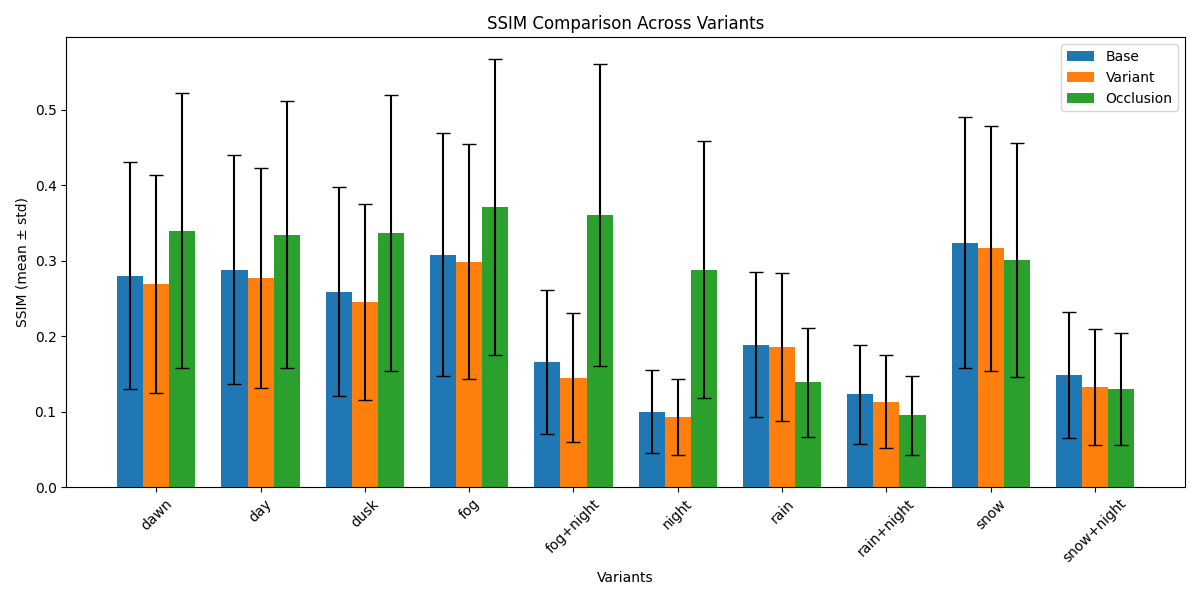
\includegraphics[width=1.5\textwidth]{figures/SSIM.png}
  \caption{SSIM Comparison Across Variants and Datasets}
\label{fig:noise_to_image}
\end{figure}

These are positive results, clearly indicating that the data augmentation process is functioning as expected. 
The generated images are positively correlated with the template images---as expected in a data augmentation pipeline---while the similarity significantly drops as diversity is introduced.

\FloatBarrier
\section{Experimental Evaluation}

Following the methodology of \cite{voetman_big_2023}, for extrinsic evaluation, several pre-trained segmentation models are fine-tuned, comparing their performance when trained exclusively on the synthetic images of LARD \cite{ducoffe_lard_2023} and when trained on the project's datasets.

To validate the performance of the trained models, the human-labeled real images of the LARD dataset are used. The real images in LARD are divided into two folders: \emph{nominal cases} and \emph{edge cases}, the latter containing images with poor runway visibility.

Three pre-trained models from the YOLO v11 family are fine-tuned: YOLO11n (``n'' for nano), YOLO11s (``s'' for small), and YOLO11m (``m'' for medium). The larger models YOLO11l and YOLO11x were not trained due to hardware constraints.

YOLO reports metrics for two tasks: detection (bounding box evaluation) and
segmentation (segmentation mask evaluation). The metric used to compare the
performance is mAP (mean Average Precision), which is the average of the
precision-recall curve. The mAP is calculated at three different IoU (Intersection over Union) thresholds: 50\%, 75\%, and 50:95.

Two tables (Tables~\ref{tab:nominal_results} and~\ref{tab:edge_cases_results}) are presented, one for the nominal dataset and another for the edge
cases dataset. The tables show the performance of the models when trained on the
LARD dataset and the GARD datasets, with the differences in performance
highlighted, with a positive value indicating an improvement in performance of
the model trained on the GARD dataset over the comparable one with the LARD dataset.

Based on the experimental evaluation metrics, the results are overwhelmingly
positive, as the GARD dataset has consistently 
matched or outperformed the LARD dataset in most cases. Especially in the
Edge Cases dataset, which is the most challenging, the GARD dataset shows
outpeformance across all models, tasks (detection and segmentation), and mAP
thresholds.

\medskip

\begin{table}[htbp]
\centering
\small
\setlength{\tabcolsep}{4pt}
\renewcommand{\arraystretch}{1.2}

  \caption{Validation with real images from LARD dataset, \emph{Nominal} dataset: YOLO11n/s/m performance comparison between LARD and GARD variants, with per-variant differences ($\Delta$).}
  \label{tab:nominal_results}

\begin{tabular}{|c|c|ccc|ccc|}
\hline
\multirow{2}{*}{\textbf{Model}} &
\multirow{2}{*}{\textbf{Dataset}} &
\multicolumn{3}{c|}{\textbf{Detection (mAP)}} &
\multicolumn{3}{c|}{\textbf{Segmentation (mAP)}} \\
& & @50:95 & @50 & @75 & @50:95 & @50 & @75 \\

\hline
\multirow{6}{*}{YOLO11n}
& Baseline (LARD) & 0.691 & 0.862 & 0.790 & 0.485 & 0.833 & 0.507 \\
& GARD BaseImages & 0.722 & 0.874 & 0.796 & 0.452 & 0.828 & 0.441 \\
& $\Delta$ & \textbf{+0.031} & \textbf{+0.012} & \textbf{+0.006} & \textbf{-0.033} & \textbf{-0.005} & \textbf{-0.066} \\
& GARD VariantImages & 0.735 & 0.888 & 0.807 & 0.471 & 0.842 & 0.472 \\
& $\Delta$ & \textbf{+0.044} & \textbf{+0.026} & \textbf{+0.017} & \textbf{-0.014} & \textbf{+0.009} & \textbf{-0.035} \\
& GARD VariantWithOcclusion & 0.728 & 0.899 & 0.794 & 0.469 & 0.841 & 0.467 \\
& $\Delta$ & \textbf{+0.037} & \textbf{+0.037} & \textbf{+0.004} & \textbf{-0.016} & \textbf{+0.008} & \textbf{-0.040} \\
\hline

\hline
\multirow{6}{*}{YOLO11s}
& Baseline (LARD) & 0.709 & 0.870 & 0.807 & 0.498 & 0.842 & 0.526 \\
& GARD BaseImages & 0.747 & 0.894 & 0.819 & 0.454 & 0.843 & 0.432 \\
& $\Delta$ & \textbf{+0.038} & \textbf{+0.024} & \textbf{+0.012} & \textbf{-0.044} & \textbf{+0.001} & \textbf{-0.094} \\
& GARD VariantImages & 0.780 & 0.915 & 0.846 & 0.485 & 0.873 & 0.482 \\
& $\Delta$ & \textbf{+0.071} & \textbf{+0.045} & \textbf{+0.039} & \textbf{-0.013} & \textbf{+0.031} & \textbf{-0.044} \\
& GARD VariantWithOcclusion & 0.771 & 0.914 & 0.845 & 0.481 & 0.870 & 0.476 \\
& $\Delta$ & \textbf{+0.062} & \textbf{+0.044} & \textbf{+0.038} & \textbf{-0.017} & \textbf{+0.028} & \textbf{-0.050} \\
\hline


\hline
\multirow{6}{*}{YOLO11m}
& Baseline (LARD) & 0.742 & 0.906 & 0.841 & 0.512 & 0.870 & 0.529 \\
& GARD BaseImages & 0.747 & 0.889 & 0.825 & 0.452 & 0.836 & 0.434 \\
& $\Delta$ & \textbf{+0.005} & \textbf{-0.017} & \textbf{-0.016} & \textbf{-0.060} & \textbf{-0.034} & \textbf{-0.095} \\
& GARD VariantImages & 0.792 & 0.923 & 0.854 & 0.489 & 0.874 & 0.490 \\
& $\Delta$ & \textbf{+0.050} & \textbf{+0.017} & \textbf{+0.013} & \textbf{-0.023} & \textbf{+0.004} & \textbf{-0.039} \\
& GARD VariantWithOcclusion & 0.789 & 0.922 & 0.860 & 0.485 & 0.878 & 0.481 \\
& $\Delta$ & \textbf{+0.047} & \textbf{+0.016} & \textbf{+0.019} & \textbf{-0.027} & \textbf{+0.008} & \textbf{-0.048} \\
\hline

\end{tabular}
\end{table}


\begin{table}[htbp]
\centering
\small
\setlength{\tabcolsep}{4pt}
\renewcommand{\arraystretch}{1.2}
  \caption{Validation with real images from LARD dataset, \emph{Edge cases} dataset: YOLO11n/s/m performance comparison between LARD and GARD variants, with per-variant differences ($\Delta$).}
  \label{tab:edge_cases_results}

\begin{tabular}{|c|c|ccc|ccc|}
\hline
\multirow{2}{*}{\textbf{Model}} &
\multirow{2}{*}{\textbf{Dataset}} &
\multicolumn{3}{c|}{\textbf{Detection (mAP)}} &
\multicolumn{3}{c|}{\textbf{Segmentation (mAP)}} \\
& & @50:95 & @50 & @75 & @50:95 & @50 & @75 \\

\hline
\multirow{6}{*}{YOLO11n}
& Baseline (LARD) & 0.543 & 0.708 & 0.634 & 0.399 & 0.700 & 0.414 \\
& GARD BaseImages & 0.608 & 0.802 & 0.663 & 0.425 & 0.762 & 0.439 \\
& $\Delta$ & \textbf{+0.065} & \textbf{+0.094} & \textbf{+0.029} & \textbf{+0.026} & \textbf{+0.062} & \textbf{+0.025} \\
& GARD VariantImages & 0.627 & 0.819 & 0.702 & 0.452 & 0.786 & 0.476 \\
& $\Delta$ & \textbf{+0.084} & \textbf{+0.111} & \textbf{+0.068} & \textbf{+0.053} & \textbf{+0.086} & \textbf{+0.062} \\
& GARD VariantWithOcclusion & 0.633 & 0.850 & 0.702 & 0.456 & 0.805 & 0.465 \\
& $\Delta$ & \textbf{+0.090} & \textbf{+0.142} & \textbf{+0.068} & \textbf{+0.057} & \textbf{+0.105} & \textbf{+0.051} \\
\hline

\hline
\multirow{6}{*}{YOLO11s}
& Baseline (LARD) & 0.530 & 0.696 & 0.620 & 0.395 & 0.680 & 0.388 \\
& GARD BaseImages & 0.638 & 0.834 & 0.689 & 0.440 & 0.795 & 0.446 \\
& $\Delta$ & \textbf{+0.108} & \textbf{+0.138} & \textbf{+0.069} & \textbf{+0.045} & \textbf{+0.115} & \textbf{+0.058} \\
& GARD VariantImages & 0.686 & 0.859 & 0.772 & 0.476 & 0.827 & 0.490 \\
& $\Delta$ & \textbf{+0.156} & \textbf{+0.163} & \textbf{+0.152} & \textbf{+0.081} & \textbf{+0.147} & \textbf{+0.102} \\
& GARD VariantWithOcclusion & 0.681 & 0.883 & 0.735 & 0.470 & 0.830 & 0.478 \\
& $\Delta$ & \textbf{+0.151} & \textbf{+0.187} & \textbf{+0.115} & \textbf{+0.075} & \textbf{+0.150} & \textbf{+0.090} \\
\hline

\hline
\multirow{6}{*}{YOLO11m}
& Baseline (LARD) & 0.551 & 0.730 & 0.653 & 0.406 & 0.719 & 0.396 \\
& GARD BaseImages & 0.641 & 0.826 & 0.702 & 0.433 & 0.791 & 0.429 \\
& $\Delta$ & \textbf{+0.090} & \textbf{+0.096} & \textbf{+0.049} & \textbf{+0.027} & \textbf{+0.072} & \textbf{+0.033} \\
& GARD VariantImages & 0.684 & 0.863 & 0.747 & 0.477 & 0.813 & 0.494 \\
& $\Delta$ & \textbf{+0.133} & \textbf{+0.133} & \textbf{+0.094} & \textbf{+0.071} & \textbf{+0.094} & \textbf{+0.098} \\
& GARD VariantWithOcclusion & 0.700 & 0.887 & 0.770 & 0.484 & 0.842 & 0.492 \\
& $\Delta$ & \textbf{+0.149} & \textbf{+0.157} & \textbf{+0.117} & \textbf{+0.078} & \textbf{+0.123} & \textbf{+0.096} \\
\hline

\end{tabular}
\end{table}

\FloatBarrier
\section{Discussion}

One concern with validating trained models with the Nominal dataset is that
images from this same dataset were used as template images for the data
augmentation pipeline. This might have introduced a bias in the evaluation, as
the generated images are based on the same structure as the template images.
But, we can be confident that either there is no bias or that the bias is
minimal, as the SSIM results show positive, but small correlation score between
the template images and the generated images. Another reason why this should not
be a concern is that the fine-tuned models performed better in the Edge Cases dataset, of which no images were used in the data augmentation pipeline.

Another limitation of the experimental evaluation setup was that the models were
fine-tuned on each isolated GARD dataset, without mixing them. This might have
limited the performance of the models, as each dataset has distinct features
that could have increased the diversity of a mixed dataset.

The better performance of the LARD-based models in the Nominal dataset might be
explained by the fact that the LARD dataset contains low diversity of weather
and lighting conditions, and runway occlusion, which matches the characteristics
of the Nominal dataset. This highlights the \emph{joint hypothesis problem} that
was presented in the literature review section.

This is also corroborated by the better performance of the GARD-based models in
the Edge Cases dataset, where the better diversity and realism of the GARD
datasets allowed the models to generalize better to the unseen data.

Because of time and hardware constraints, the evaluation was limited to the
YOLO11 family of models. Future work could include more models, and more
complex pipelines dedicated for runway segmentation, such as VALNet
\cite{wang_valnet_2024}.

These results are promising, showing that the Canny2Concrete pipeline is
effective in generating realistic runway images that can be used to train
detection and segmentation models, and that the GARD datasets is a viable
alternative to existing synthetic datasets.

The biggest limitation in the Cany2Concrete pipeline is the need for template
images. This limits the variety of structures that can be generated, and require
a manual selection of images. Future work could be done in either
programatically generating canny edge images without extracting them from any
given image. It would also help if the diffusion model understood better the
concept of a aerial view of a runway, so that it wouldn't need detailed canny
edges to generate a realistic image.

Another limitation is that, due to the chosen Stable Diffusion model, the
images don't look as real photos, but more like digital art. Future work could
shrink "Sim2Real" gap. This could be done by using a different diffusion model,
or by adding another module to the pipeline that would convert images to this
more realistic style.

The pipeline could also generate better results by improving the outpainting
techniques used in the variant image generation module. The current techniques
generate noticeable borders between the original image and the outpainted
background.


